\documentclass{ximeraXloud}

\title{Pre-Requisites}
%%%% List of skills:
%    Arithmetic with fractions and (up to) three digit numbers without using a calculator.
%    Isolating a variable in a multivariable linear equality.
%    Correctly distributing expressions and combining like terms.
%    Interval notation.
%    Graphing points on an x-y plane, and writing the coordinates of the points on an x-y plane.
%    Order of Operations.
%    Fraction Vocabulary and fluency.

\input{../preamble}



\begin{document}
\begin{abstract}
This section covers the skills that a MAC1140 student is expected to be \textbf{fluent} in.
\end{abstract}
\maketitle

An introductory MAC1140 student should be fluent in the skills necessary to correctly answer all of the following problems. In particular, this page should take less than 35 minutes to finish, from the time a student begins the problems. If you find you are struggling to complete these problems (either at all, or in time), you should \textbf{strongly} consider dropping back to MAC1105 to review these skills and problem types before taking this course. A student that cannot complete this page with 100\% accuracy within 35 minutes has a very low chance of getting an acceptable grade in MAC1140.

\begin{problem}% Arithmetic with numbers
    Perform the following operations \textbf{without using a calculator}.
    \begin{itemize}
        \item $17 + 21 = \answer{38}$
        \item $213 + 389 = \answer{602}$
        \item $17 \times 3 = \answer{51}$
        \item $22 \times 34 = \answer{748}$
        \item $98 \div 7 = \answer{14}$
        \item $252 \div 6 = \answer{42}$
        \item $\frac{33}{5} + \frac{12}{5} = \answer{9}$
        \item $\frac{22}{3} + \frac{12}{7} = \answer{\frac{190}{21}}$
        \item $13 \cdot \frac{13}{7} = \answer{\frac{169}{7}}$
        \item $\frac{12}{5} \div \frac{5}{6} = \answer{\frac{72}{25}}$
        \item $3(2 + 7) - 9 = \answer{18}$
        \item $3 - 2(5 - 1) + 1 = \answer{-4}$
        \item $12 + 2\cdot 3 - 12\div 4 = \answer{15}$
    \end{itemize}
\end{problem}

\begin{problem}% Solving linear functions for a single variable.
    Solve the following equations for the specified variable.
    \begin{itemize}
        \item Solve for $x$: $3x + 2y = 17$. Then $x = \answer{\frac{17-2y}{3}}$.
        \item Solve for $a$: $13a + 3(2a - 7b) + 10b = 2a$. Then $a = \answer{\frac{11b}{17}}$
        \item Solve for $r$: $-4(3 - q) + 12r = 13(q + 1)$: Then $r = \answer{\frac{9q+25}{12}}$ 
        \item Solve for $d$: $3a - 21b - 3(b + c + d) = 12$: Then $d = \answer{a - 8b-c-4}$
    \end{itemize}
\end{problem}

\begin{problem}% Correctly Distributing binomial expressions
    For the following problems, expand everything fully, then enter in the resulting coefficients in front of each variable. For example:
    \[
        (x + y)(3x + 22) = 3x^2 + 3xy + 22x + 22y = (3) \cdot x^2 + (3) \cdot xy + (22) \cdot x + (22) \cdot y
    \]
    
    \begin{itemize}
        \item $3(x + 7) = \answer{3} \cdot x + \answer{21}$
        \item $-2(12x - 3y) = \answer{-24}\cdot x + \answer{6}\cdot y$
        \item $(2 - x)(3 + y) = \answer{-1}\cdot xy + \answer{-3}\cdot x + \answer{2} \cdot y + \answer{6}$
    \end{itemize}
\end{problem}

\begin{problem}% Interval Notation
    For the following problems, select the correct interval notation options to reflect the written expression.
    \begin{itemize}
        \item ``All real numbers strictly between $3$ and $7$.'' \wordChoice{\choice[correct]{$(3$}\choice{$[3$}\choice{$(7$}\choice{$[7$}},\wordChoice{\choice{$3)$}\choice{$3]$}\choice[correct]{$7)$}\choice{$7]$}}.
        \item ``Real numbers that are, at most, seven.''
        \wordChoice{\choice[correct]{$(-\infty$}\choice{$[-\infty$}\choice{$(\infty$}\choice{$[\infty$}\choice{$(7$}\choice{$[7$}\choice{$(-7$}\choice{$[-7$}},\wordChoice{\choice{$-\infty)$}\choice{$-\infty]$}\choice{$\infty)$}\choice{$\infty]$}\choice{$7)$}\choice[correct]{$7]$}\choice{$-7)$}\choice{$-7]$}}.
    \end{itemize}
\end{problem}

\begin{problem}% Vocabulary
    Consider the fraction $\frac{3}{7}$. \\
    What is the Numerator? $\answer{3}$. What is the Denominator? $\answer{7}$.
    
\end{problem}

\begin{problem}
    Consider the following graph:
    \begin{center}
        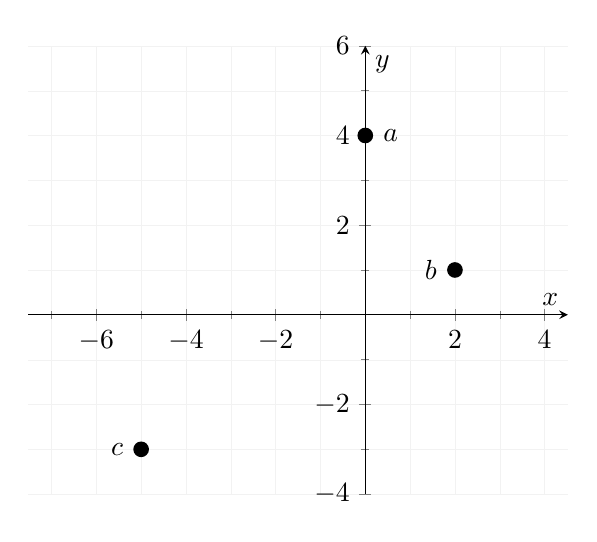
\begin{tikzpicture}
            \begin{axis}[
                    axis x line=middle, 
                    axis y line=middle, 
                    xlabel={$x$}, 
                    ylabel={$y$}, 
                    axis equal, 
                    grid=both, 
                    grid style={line width=.1pt, draw=gray!10}, 
                    minor tick num=1, 
                    ymax=6, 
                    ymin=-4
                ]

                \addplot[mark=*,only marks] coordinates {(2,1)(-5,-3)(0,4)};
                \node[label={180:{$b$}},circle,fill,inner sep=2pt] at (axis cs:2,1) {};
                \node[label={180:{$c$}},circle,fill,inner sep=2pt] at (axis cs:-5,-3) {};
                \node[label={0:{$a$}},circle,fill,inner sep=2pt] at (axis cs:0,4) {};
            \end{axis}
        \end{tikzpicture}
    \end{center}
    
    \begin{itemize}
        \item What are the coordinates of $a$? $(\answer{0},\answer{4})$
        \item What are the coordinates of $b$? $(\answer{2},\answer{1})$
        \item What are the coordinates of $c$? $(\answer{-5},\answer{-3})$
    \end{itemize}
\end{problem}


\end{document}